\section{Evolution}
\label{sec:iterative-dsl-evolution:SLCO_Evolution}
Van Deursen et al.\ identify three phases in the development of a DSL: the analysis phase, the implementation phase, and the phase in which the DSL is used~\cite{Deursen2000}.
Mernik et al.\ split the analysis phase into an analysis and a design phase~\cite{Mernik2005}.
Because the development of our language is an iterative process, the phases are revisited each time the language is extended.
The evolution of the language and the transformations has been influenced by a number of roles, each of which is responsible for performing certain activities that belong to the four phases in the development of a DSL mentioned above.
We describe the evolution of our DSML and the accompanying transformations in terms of the activities performed during these four phases.
The remainder of this section starts with a description of the roles and the activities that belong to these roles.
After these descriptions, the major changes made in both the language and the transformations are listed.
At the end of this section, we cluster these changes and distinguish four types of causes for evolution.

\subsection{Roles and Activities}
\label{sec:iterative-dsl-evolution:SLCO_Evolution_Roles}

The design of our DSML has been influenced by a number of roles.
Table~\ref{tab:roles_phases} shows in which phases of the development each of the roles participate.
Although every role has its own separate tasks, these tasks greatly depend on each other, which leads to interaction between the roles.
In the evolution of our DSML, language designers, platform experts, modelers, and software developers have played a role.

\begin{table}[hbt]
\centering
\small
\begin{tabular}{|l|l|}
\hline
\rowcolor[gray]{.9}
\textbf{Development phases} & \textbf{Roles} \\
\hline
\multirow{2}{*}{Analysis}   & Language designer \\
                            & Platform expert \\
\hline
Design                      & Language designer \\
\hline
Implementation              & Software developer \\
\hline
Use                         & Modeler \\
\hline
\end{tabular}
\caption{Development phases and the corresponding roles}
\label{tab:roles_phases}
\end{table}

Table~\ref{tab:roles_activities} shows how the aforementioned roles are related to activities and the number of persons that fulfilled the roles.
The actual number of modelers is larger than shown in the table.
\SLCO has been used in a number of student assignments in which students had to create models.
However, little to no feedback was acquired from the students.
Because their influence on the evolution of \SLCO is negligible, they are not explicitly mentioned in the table.
Below, we describe how the roles and activities relate.

In our development process, language designers are involved in two activities.
First, they perform a domain analysis to investigate which aspects of the problem domain need to be incorporated in the language.
After the domain analysis is completed and all the concepts that need to be incorporated in the DSML have been identified, the language designers are responsible for defining the syntax and semantics of the language.

\begin{table}[hbt]
\centering
\small
\begin{tabular}{|l|c|l|}
\hline
\rowcolor[gray]{.9}
\textbf{Role}                       & \textbf{Persons}   & \textbf{Activities} \\
\hline
\multirow{2}{*}{Language designer}  & \multirow{2}{*}{4} & Domain analysis \\
                                    &                    & Defining the language \\
\hline
\multirow{3}{*}{Platform expert}    & \multirow{3}{*}{4} & Domain analysis \\
                                    &                    & Defining the mapping from \SLCO to a platform \\
                                    &                    & Interpreting models \\
\hline
\multirow{3}{*}{Modeler}            & \multirow{3}{*}{3} & Creating models \\
                                    &                    & Applying transformations \\
                                    &                    & Interpreting models \\
\hline
\multirow{2}{*}{Software developer} & \multirow{2}{*}{2} & Implementing the mappings \\
                                    &                    & Implementing editors for \SLCO models\\
\hline
\end{tabular}
\caption{Roles and the corresponding activities}
\label{tab:roles_activities}
\end{table}

\SLCO models are transformed to a number of platforms.
Support for these target platforms was added one at a time, and in some cases, adding a new platform changed the application domain of the language.
This is caused by our decision to extend the language whenever necessary such that it is suited for modeling on both high and low levels of abstraction.
For example, to be able to use \SLCO to model systems on the level of abstraction offered by \NQC, the concept of asynchronous communication was added to the language.
Each time changes like this have to be made, the platform expert performs an additional analysis of the domain of the language.
Platform experts are also responsible for the mapping from \SLCO to new target platforms.
This mapping defines how constructs of the DSML are mapped onto constructs available for the target platform.
In some cases, not all constructs need to have an equivalent counterpart in the target platform.
The language and tools offered by the target platform have a certain purpose, and some constructs of \SLCO may be irrelevant for the purpose of the target platform.
%The expert investigates whether all constructs of \SLCO have a counterpart on the target platform.
%If such counterparts do not exist and cannot be simulated using other constructs, the platform expert and the language designer will consider whether the source language needs to be adapted.
Lastly, platform experts may be involved in the interpretation of models.
For example, a \Spin expert was asked to analyze a number of \SLCO models that suffered from state-space explosion after translating them to \Promela and processing them with \Spin.
Based on the advice of this expert, both the language and the model transformations were changed.
In our case, a \POOSL expert, \Spin experts, and \NQC experts participated in the development of the language.

The modeler is the end-user of a DSML.
Besides creating models and generating new models by applying transformations, the modeler analyzes and interprets models.
To simulate an \SLCO model, for example, the modeler can transform this model to an equivalent \POOSL model.
This \POOSL model can then be simulated, after which the results of the simulation have to be interpreted to determine their relevance for the original \SLCO model.

Given a mapping from \SLCO to a target platform designed by a platform expert, software developers are responsible for the translation of the conceptual mapping to an actual implementation of the transformation.
Furthermore, the software developers implement the editors required for creating and editing models.

\subsection{Evolution of the Language}
\label{subsec:iterative-dsl-evolution:evolution}
While performing the activities described in Section~\ref{sec:iterative-dsl-evolution:SLCO_Evolution_Roles}, various features were identified and added to the language.
Table~\ref{tab:activities_changes} shows how the activities are related to these features.
Each of the features is discussed in the remainder of this section.

\begin{table}[hbt]
\centering
\small
\begin{tabular}{|l|l|}
\hline
\rowcolor[gray]{.9}
\textbf{Activity}                          & \textbf{Language features} \\
\hline
\multirow{5}{*}{Domain analysis}           & Concurrent, communicating objects \\
                                           & Simple imperative constructs \\
                                           & Delays \\
                                           & Asynchronous signals \\
                                           & Lossy channels \\
\hline
\multirow{3}{*}{Defining the language}     & UML-like syntax \\
                                           & Synchronous signals \\
                                           & Subset for formal semantics \\
\hline
\multirow{8}{*}{Interpreting models}       & Conditional signal reception \\
                                           & Combination of trigger and guard \\
                                           & Local variables \\
                                           & Structure diagrams \\
                                           & Additional operators and types \\
                                           & Incoming transitions for initial states \\
                                           & Outgoing transitions for final states \\
                                           & Fine-grained sequences of transformations \\
\hline
\multirow{4}{*}{Creating models}           & Initial values of variables \\
                                           & Identifying signals by name \\
                                           & Textual syntax \\
                                           & Generalization of statements, triggers, and guards \\
\hline
\multirow{2}{*}{Implementing the mappings} & Explicit channel types \\
                                           & Restricted form of conditional signal reception \\
\hline
\end{tabular}
\caption{Desired language features identified during each of the activities}
\label{tab:activities_changes}
\end{table}

%% Domain analysis
% OK Concurrent communicating objects
% OK Simple imperative constructs
% OK Delays
% OK Asynchronous signals
% OK Lossy channels
From an abstract point of view, the problem domain for which \SLCO was designed consists of concurrent, communicating objects.
The most important requirement for our DSML is therefore that it can describe such objects at an appropriate level of abstraction.
The initial application area of \SLCO was performance analysis of interoperating software components implemented with an imperative programming language.
Besides communicating with each other, these components perform simple calculations.
To be able to express the calculations performed by the components, a small number of basic imperative constructs were added to the language.
Furthermore, to enable performance analysis, time needed to be incorporated into the language, which was achieved by adding delay statements.
All of these aspects of the language were identified during the initial analysis of the problem domain.
At a later stage, the aspiration to execute \SLCO models on the Lego Mindstorms platform gave rise to a second analysis of the problem domain.
Communication between RCXs, the controllers of the Lego Mindstorms platform, occurs using infrared signals.
These signals are asynchronous, and the channel used for this type of communication is unreliable.
Initially, communication in \SLCO could only occur using synchronous channels over reliable channels, as explained below.
To enable a straightforward mapping from \SLCO to \NQC, the characteristics of both languages should be aligned.
Therefore, \SLCO was extended with asynchronous signals and lossy channels as a result of the additional domain analysis.

\begin{figure}[hbt]
\centering
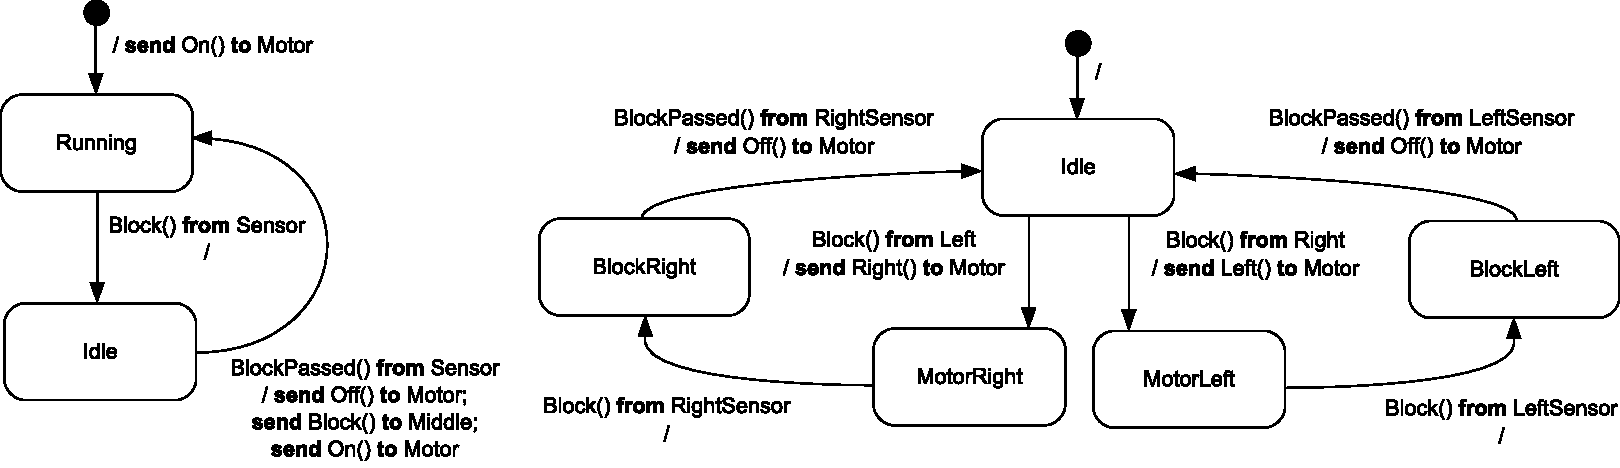
\includegraphics[scale=.49]{iterative-dsl-evolution/figs/middle_left_right}
\caption{Syntax that distinguishes triggers, guards, and statements}
\label{fig:iterative-dsl-evolution:old_syntax}
\end{figure}

% Defining the language
% OK UML-like syntax
% OK Synchronous signals
% OK Subset for formal semantics
One purpose of \SLCO is using the language for documentation.
For this reason, a graphical syntax resembling the well-known syntax of the \UML was chosen while defining the language.
Another design decision we made for this reason is offering communication via synchronous signals.
This form of communication leads to concise models, which increases the understandability of models and thus increases their value as documentation.
In Figure~\ref{fig:iterative-dsl-evolution:old_syntax}, two state machines are shown using the graphical syntax that was inspired by the \UML.
Over time, this syntax has changed a little, as is explained below.
Finally, to simplify the definition of \SLCO's formal semantics, a sublanguage has been identified, which is described in Section~\ref{sec:SLCO:simplified_slco}.
Because each of the constructs that are missing from this sublanguage can be expressed in terms of its other constructs, \SLCO's semantics can be defined completely by defining the semantics of this sublanguage only.


% Interpreting models
% OK Conditional signal reception
% OK Combination of trigger and guard

% OK Local variables
% OK Structure diagrams
% OK Additional operators and types

% OK Incoming transitions for initial states
% OK Outgoing transitions for final states

% NVT Fine-grained transformations

\begin{figure}[hbt]
  \centering
  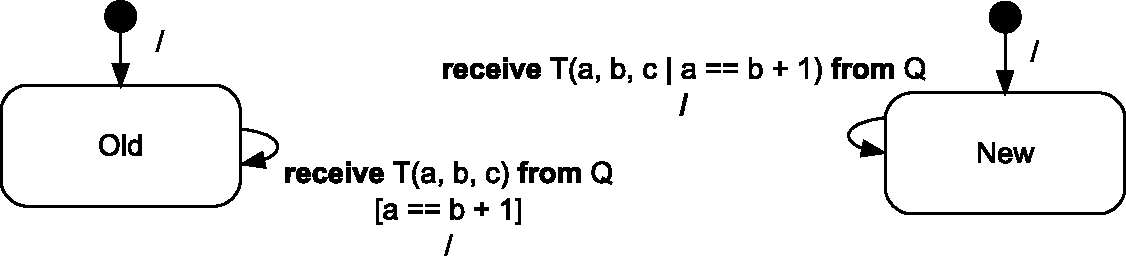
\includegraphics[scale=.40]{iterative-dsl-evolution/figs/cond_before_after}
  \caption{Evolution of conditional signal reception}
  \label{fig:iterative-dsl-evolution:cond_before_after}
\end{figure}

Many of the changes to the language were inspired by problems encountered during the interpretation of models.
During the interpretation of \Promela models, for example, we noticed that the state space generated as part of the model-checking process could be reduced by adapting the language.
Because reducing the state space improves verification performance, we adapted \SLCO by introducing conditional signal reception as a language construct.
Conditional signal reception can be used to specify that a signal can only be received if its arguments adhere to a certain condition.
The leftmost transition from state~\SLCOState{Old} to itself in Figure~\ref{fig:iterative-dsl-evolution:cond_before_after}, for example, will only be taken when a signal~\SLCOSignal{T}{a, b, c} is received for which the condition~$a==b+1$ holds.
The original syntax used for this construct was again inspired by the \UML.
The fact that the variables used in the guard~$a==b+1$ refer to the values received as arguments of signal~\SLCOSignalName{T} proved to be a source of confusion that was addressed at a later stage.
The condition was incorporated into the language construct for signal reception, as shown on the right of Figure~\ref{fig:iterative-dsl-evolution:cond_before_after}.

During the interpretation of \SLCO models, we noticed that some variables were used only locally in the state machines, but were defined globally as variables of the class containing the state machines.
To improve the readability of the models, we introduced the concept of local variables.
However, this increase in readability is accompanied by a decrease in modifiability when using the standard tree view editor provided by the Eclipse Modeling Framework (EMF)~\cite{Steinberg2008} for editing models.
When referring to a variable in this tree view editor, the container of a variable is not shown in the list of variables that can be referred to.
This makes it hard to distinguish between two variables with the same name but with a different container.
The readability of models was also improved by extending the graphical syntax with structure diagrams.
These diagrams make it possible to visualize all aspects of an \SLCO model.
They provide information about models that was missing from the communication and behavior diagrams, such as the scope and initial value of variables.
Another improvement in terms of readability and modifiability we made after interpreting \SLCO models is adding new operators and types to the language.

Once the state spaces of \SLCO models could be visualized with the executable prototype of \SLCO's semantics presented in Chapter~\ref{chap:prototype-semantics}, the fact that initial states were not allowed to have incoming transitions and final states were not allowed to have outgoing transition showed to clutter the graphs that represented the state spaces.
Therefore, we removed these restrictions and changed the way initial and final states are shown in behavior diagrams.
Previously, both the solid black circles as well as the rounded rectangles in behavior diagrams, such as the ones shown in Figure~\ref{fig:iterative-dsl-evolution:cond_before_after}, represented states.
After the aforementioned restrictions were removed, a solid black circle no longer represents a separate state.
Instead, the black circle is now only used to indicate which of the rounded rectangles represents an initial state.
The way final states are displayed changed similarly.
Table~\ref{tab:activities_changes} also indicates that the transformations have changed as a result of problems that occurred while interpreting models.
These changes are discussed in Section~\ref{subsec:iterative-dsl-evolution:trafo}.

% Creating models
% OK - Initial values of variables
% OK - Identifying signals by name
% OK - Textual syntax
% OK Generalization of statements, triggers, and guards

The activity of creating models inspired four changes.
While creating models, we noticed that it was tedious to initialize variables explicitly as part of a state machine describing the behavior of a class.
For this reason, we made it possible to specify the initial value of a variable as part of its declaration.
Another design decision that was tedious to deal with while creating models by hand was the existence of a metaclass for signals.
In the current version of \SLCO, this metaclass is replaced with a simple attribute of type String that denotes the name of a signal.
Additionally, the textual syntax for \SLCO was introduced because of difficulties encountered while creating models.
Besides offering a more convenient way to create and edit models, the textual representation was also a prerequisite for the work presented in Chapter~\ref{chap:prototype-semantics}.
Finally, the distinction between guards, triggers, and statements was removed.
Early versions of \SLCO distinguish between guards, triggers, and statements, as is the case for the \UML.
Furthermore, each transition has at most one guard, at most one trigger, and can have any number of statements.
Allowing at most one trigger and guard per transition can lead to models with a large number of states.
To reduce the number of states, the distinction between guards, triggers, and statements was removed.
Figure~\ref{fig:slco:ConveyorSMS} shows the state machines of Figure~\ref{fig:iterative-dsl-evolution:old_syntax} using the new syntax.

\begin{figure}[hbt]
  \centering
  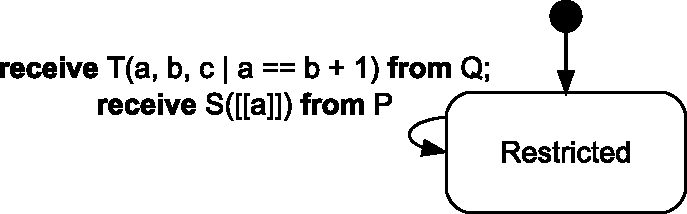
\includegraphics[scale=.40]{iterative-dsl-evolution/figs/cond_promela}
  \caption{Restricted form of conditional signal reception}
  \label{fig:iterative-dsl-evolution:cond_promela}
\end{figure}

% Implementing the mappings
% OK Explicit channel types
% OK Restricted form of conditional signal reception
Implementing the mappings from \SLCO to its target platforms led to two changes.
In \SLCO, the arguments of all signals sent over a channel must have the same type.
A channel in \SLCO is characterized by these types, its directionality, its reliability, and its suitability for either synchronous or asynchronous communication.
Initially, the allowed types of the arguments and the directionality of a channel were left implicit.
However, the types of the arguments of the signals sent over a channel must be specified explicitly in \Promela.
When transforming \SLCO to \Promela, the characteristics of a channel had to be derived from the statements that use the channel for sending and receiving signals.
To avoid this, we decided to make all the characteristics of channels explicit, which led to smaller transformations that were easier to understand and modify.
Furthermore, while investigating different forms of conditional signal reception and their mapping to the target platforms, we noticed that only some of these forms could be translated to \Promela.
The signal reception with the condition $a == b + 1$ shown in Figure~\ref{fig:iterative-dsl-evolution:cond_promela}, for instance, has no counterpart in \Promela that matches the semantics of \SLCO.
To simplify the implementation of the mapping from \SLCO to \Promela, we introduced a restricted form of conditional signal reception, which corresponds directly with \Promela's construct for conditional signal reception.
The statement~\SLCOSignalReception{S}{[[a]]}{P} in Figure~\ref{fig:iterative-dsl-evolution:cond_promela}, for example, can be translated to \Promela straightforwardly.

Defining the mappings from \SLCO to the various target platforms and implementing the editors for \SLCO models did not lead to any modifications of the language.
However, as stated before, additional domain analysis was performed by the platform experts before defining the mappings to the target platforms.
The straightforwardness of these mappings is caused by the extension of \SLCO that resulted from the additional domain analysis.

\subsection{Evolution of the Transformations}
\label{subsec:iterative-dsl-evolution:trafo}
The transformations from \SLCO to the various platforms have also evolved.
One reason for this evolution was the decision to divide each transformation into steps that either modify existing elements of a model or add elements to a model.
We chose this approach because it clarifies the relation between two consecutive steps of a sequence of transformation.
It is now easier to see what has changed after applying a single transformation.

\begin{figure}[hbt]
 \centering
 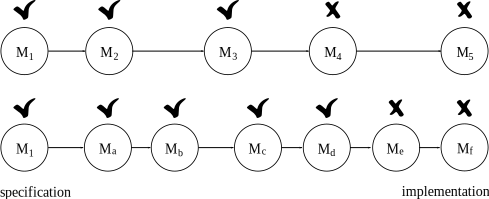
\includegraphics[width=.7\columnwidth]{iterative-dsl-evolution/figs/fine-grained-transformations}
 \caption{A coarse-grained and a fine-grained sequence of transformations}
 \label{fig:iterative-dsl-evolution:fine-grained-transformations}
\end{figure}

Another reason for splitting up some of the transformations into smaller steps is to enable verification of intermediate models that are closer to the implementation.
This is schematically depicted in Figure~\ref{fig:iterative-dsl-evolution:fine-grained-transformations}.
Before splitting the transformations into smaller parts, models~\Model{1}, \Model{2}, and~\Model{3} could be verified using model checking.
Verifying model~\Model{4} was already impossible due to the state-space explosion problem.
After splitting, verification up to model~\Model{d} is possible.
This model is much closer to the implementation than model~\Model{3}.
Splitting the transformations increased the usability of the models.

\subsection{Generalization}
Looking more closely at the evolution of our language and transformations, we noticed that the design choices and changes can be divided into four categories.
We consider these categories to characterize the main influences on the evolution of our DSML and transformations.

The choice of defining a language for the specification of systems consisting of concurrent objects is made to effectively describe problems in the \emph{problem domain}.
The influence of the problem domain on the evolution of a DSML is to be expected, since the language is focused on that domain.

In our case, the \emph{target platforms} also have an impact on the evolution, since our language does not have its own execution platform, nor is it embedded in another language.
If a transformation to, for example, an execution platform is impossible due to language mismatches, it is impossible to execute a model created using the DSML.
Therefore, our DSML has evolved to eliminate unresolvable mismatches with the target platforms.
The introduction of conditional signal reception and the division of the transformations into smaller steps are enforced by the target platforms.

A large number of design decisions have been made to increase the \emph{quality of models}, in particular their understandability and modifiability.
Defining a graphical syntax for the language, adding synchronous communication, introducing local variables, and allowing variables to have an initial value have been done to increase the understandability.
Referring to signals based on their name has increased the modifiability of models.
The many changes required for increasing the understandability and modifiability of our DSML can be partially explained by our lack of experience in designing DSLs.
We found that it is hard to predict which language features will improve understandability and modifiability without actually using the language.
These are, however, important quality attributes that should be taken into account to enhance the chance for acceptance of the language in practice.
We expect that there are more quality attributes~\cite{Boehm1978} that influence the evolution of a language, which will become apparent when the language is used more~extensively.

Enhancing the \emph{quality of the transformations} also had its effect on the language.
To increase the understandability and modifiability of the transformations, certain implicit language features have been made explicit, such as the directionality of channels and the argument types of the signals sent over channels.
